\chapter{Background and Related Work}
\indent This chapter describes the context and background of this thesis. We first review common strategies for feature selection. We integrate causal discovery into our interactive feature selection workflow. We describe various causal discovery algorithms and representations of causal networks. Then, we explain visualizations and its use in interactive machine learning. We also describe the importance and methods for evaluating novel visualization systems. Lastly, we describe relevant works in interactive machine learning and machine learning visualization.

\section{Feature Selection}
\indent Classification is the process of creating a model that maps the input \(X=[x_1, x_2, ..., x_N]\) to output class label \(y\) and will predict $y$ of unseen data points. An example is the classification of emails as spam or not spam. The two categories or target labels are spam and not spam; possible features that can describe emails are word count, the frequency of words, location email sent from, etc. Features are measurable properties or characteristics that may help predict the target label. However, not all features are predictive of the target label, and so feature selection is often performed before creating the model. 
Feature selection is the task of selecting a subset of features in \(X\) to create a classifier that maximizes an objective which is often its prediction performance on unseen examples. The selected feature subset directly influences the created model and its performance. The three main categories for feature selection approaches are filter, wrapper, and embedded. 

\subsection{Filter Based Feature Selection}
Filter based methods evaluate individual features or feature subset based a criterion \(J\) such as information content, entropy, relevance, etc. The criterion value measures the usefulness of a feature or feature subset. The top \(k\) candidates are selected for creating the classification model. However, filter based methods may not remove redundant and irrelevant features. Also, the feature subset may not build the best performing classifier because the evaluation criterion is independent of the classifier performance.

Brown and et. al. proposed a framework that expresses the heuristic of filter algorithms in terms of mutual information \cite{Brown}. Information based criteria expresses the correlation between features and the target label. The intuition for information based criteria is that highly correlated features may be predictive of the target. Measures of information are expressed in terms of entropy, which describes the uncertainty in the distribution of a random variable \(X\). The equation for entropy of a discrete random variable $X$ is
\begin{equation}
H(X) = -\sum_{x \in X} p(x)\log p(x)
\end{equation}
where \(x\) represents the values \(X\) can take and \(p(x)\) the fraction of the observed examples taking on value \(x\) for \(X\). If \(x\) takes on mostly one value \(X\), then there is little uncertainty about the value of \(x\) and \( H(X)\) is low. On the other hand, if all values of \(X\) are equally likely then we are uncertain about the value of \(x\) and \( H(X)\) is high. The equation for conditional entropy of \(X\) given random variable \(Y\) is 
\begin{equation}
H(X|Y) = -\sum_{y \in Y} p(y) \sum_{x \in X} p(x|y)\log p(x).
\end{equation}
\(H(X|Y)\) can be explained as the amount of uncertainty in \(X\) after we learned the value of \(Y\). The equation for mutual information is 
\begin{equation}
I(X;Y)= H(X)-H(X|Y). 
\end{equation}
\(I(X;Y)\) is the difference between the entropy of \(X\) before \(Y\) is known and the entropy of \(X\) after \(Y\) is known and expresses the amount of information shared between \(X\) and \(Y\). The Mutual Information Maximization (MIM) scoring criterion ranks the features based on the amount of shared information between the feature and target $Y$. MIM is expressed as  
\begin{equation}
\label{eqn:MIM}
J_{MIM}(X_k) = I(X_k;Y). 
\end{equation}

MIM criterion can be used to describe how relevant a feature or feature subset is to the target variable. In the interactive feature selection system, MIM score of the selected feature set is graphically displayed to help the user filter for relevant feature.

\subsection{Wrapper methods for Feature Selection}
Wrapper method is the second category of feature selection approaches. One example is forward feature selection, a greedy algorithm that starts with an empty feature set and iteratively adds the feature that would most improve the classifier's performance. Wrapper methods can be used with most learning algorithms because the classifier is treated as a black box. However, the feature subset is only optimal for that specific learning algorithm. Another downside is that the search space grows with the number of features; as a result, wrapper methods are computationally expensive since the classifier has to be re-evaluated for every new feature subset. Wrapper methods are infeasible for large data sets and computationally expensive. 

\subsection{Embedded and Hybrid}
Embedded methods incorporate or embed feature selection as a part of the learning algorithm. Variants of the decision tree algorithm, such as CART and random forest, are embedded methods. Hybrid methods combine the desired properties of filter and wrapper methods. A filter is first used to reduce the feature space and then a wrapper method is used to find the best feature subset.  

\section{Causal Feature Selection} \label{CausalFSSubsection}
Causal discovery uncovers causal relationship between features for a set of \(N\) input features \(X = [x_1, x_2, ..., x_n]\). In contrast to feature selection, target variable is not singled out and any variable can be the target.  

Although conventional feature selection algorithms in machine learning literature do not uncover causal relationships between variables since it is not required for finding good predictors of the target variable, causal discovery can be advantageous for feature selection. By selecting features based on their effectiveness at predicting the target variable, feature selection algorithms may select features that are results of experimental side effects rather than properties of the studied system. Awareness of cause and effect relationships supports machine learning practitioners in selecting relevant features and increases understanding of the underlying data generation mechanisms. Moreover, causal information can increase model transparency, which can increase trust in the system and its predictions.

\subsection{Causal Bayesian Network} \label{CBN}
\begin{figure}[h]
\centering
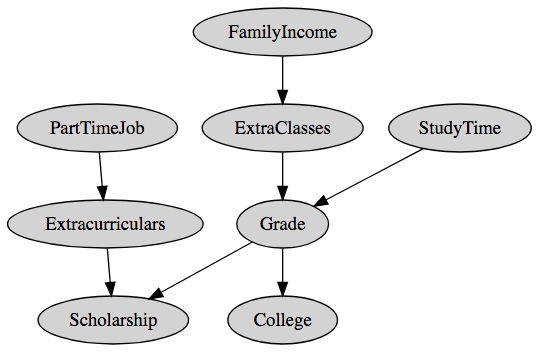
\includegraphics[width=1\textwidth]{CBN}
\caption{\textbf{Causal Bayesian Network}. A Bayesian network represents a set of variables and their conditional dependencies via a directed acyclic graph (DAG). In a causal network, edges represent causal relationships.}\label{fig:CBN}
\end{figure}

Causal Bayesian network is a framework for representing causal relationships for a set of random variables \(X = [x_1, x_2, ..., x_n]\). A Bayesian network for \(X\) consists of a directed acyclic graph (DAG) where each node maps one to one to a variable in \(X\) and a probability distribution of the nodes. The graph \(G\) imposes independence constraints that any probability distribution of the network must hold.  The Markov condition of Bayesian networks requires each node to be conditionally independent of non-descendent nodes given its parent node. In causal Bayesian networks, directed edges represent relationships between adjacent nodes. For all \(x_i\) and \(x_j\) in \(X\), if there is a directed edge from \(x_i\) to \(x_j\), feature \(x_i\) is a direct cause of feature \(x_j\). Causal Bayesian network is a map of dependencies and independencies of \(X\). 

\subsection{Markov blanket} \label{MarbovBlanket}
\begin{figure}[h]
\centering
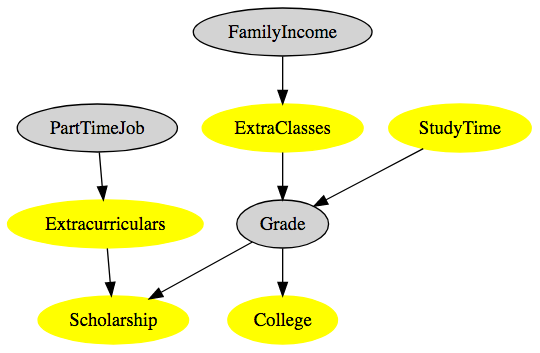
\includegraphics[width=1\textwidth]{MB}
\caption{ 
\textbf{Markov blanket.} The central node represents the variable Grade. The highlighted nodes are members of Grade's Markov blanket. Extra classes and study time are direct causes or parents; scholarship and college are direct effects or children; extracurricular is a spouse or a direct cause of its child. Given these variables, ``Grade" is independent of other variables in the graph. }\label{fig:MB}
\end{figure}
\indent The Markov blanket in a Bayesian network is the set of features that separates a given feature from the rest of the graph. The Markov blanket is composed of direct causes (parents), direct effects (children), and direct causes of direct effects (spouses). After the direct causes of the target are known, indirect causes do not provide any additional information since their effect on the target is captured in the direct causes (Markov's condition). Moreover, children of the target are predictive of the target, and knowing the other causes of the target's children (spouses) can help explain the amount of effect the target has on its children. Therefore, direct effects (children) along with the direct causes of the direct effects (spouses) enhance each other's predictive power. 

Researchers have suggested that the target's Markov blanket is an important concept for feature selection \cite{MBforCL}. Feature relevance can be described using the Bayesian network. For any feature \(Y\), an irrelevant feature is disconnected from \(Y\) in the network. Features in the Markov blanket of \(Y\) are strongly relevant features. Features that are not in the Markov blanket of \(Y\) but have a directed path to \(Y\) are weakly relevant features \cite{CausalFS}. Based on the concepts of Markov blanket and feature relevance, we can utilize causal discovery and causal Bayesian networks to identify weakly and strongly relevant features that may be predictive of the target label.

\subsection{Greedy Equivalence Search (GES)} \label{GESSubsection}
Learning Bayesian network structures from observational data have been extensively studied. One reason learning Bayesian networks is an important problem is that edges in Bayesian networks can be used to infer causal influences. One approach to the Bayesian network learning problem is the search and score method which searches the space of possible structures and evaluates models based on a scoring criterion \(S(G,D)\) that measures how well a structure $G$ fits the data $D$. GES is an implementation of the search and score method. The search evaluates the hypothesis \(G^h\) which states that the set of observed data is sampled from a distribution that exactly contains the independence constraints imposed by \(G\). The Bayesian scoring criterion \(S_B\), the log posterior of the hypothesis \(G^h\), is used to evaluate structures $G$. The scoring function is 
\begin{equation}
S_B(G,D) = logp(G^h) + logp(D|G^h) 
\end{equation} where \(p(G^h)\) is the prior probability of \(p(G^h\)) and \(p(D|G^h\)) is the likelihood of the hypothesis given the observed data. 

For two DAGs \(H\) and \(G\), \(H\) is an independence map of \(G\) if the independence implied by the structure of \(H\) is also implied by the structure of \(G\). For an independence map \(H\) of \(G\), there exist a finite sequence of edge modification that can be applied to \(G\) such that after each edge modification \(H\) is still an independence map of \(G\) and at the end of the sequence \(G = H\). \(H\), \(G\), and the intermediate DAGs \(G'\) are in the same equivalence class. Let \(\epsilon\) denote the equivalence class.

\begin{algorithm}
\caption{GES} \label{GES}
\begin{algorithmic}[1]
\Procedure{GES}{}
\State {$\epsilon \gets$ \text{Empty Network}}
\State {$currentScore = null$}
\While { $BayesianScore(\epsilon) > currentScore $}
\State {$currentScore = BayesianScore(\epsilon)$}
\State {$ EdgeAdditions \gets FindAllPossibleEdgeAdditions(\epsilon) $}
\For {$ edge \in EdgeAdditions $}
\For {$G \in \epsilon $}
\State {$ \epsilon' = AddEdge(edge, G)$}
\If { $ BayesianScore(\epsilon') > BayesianScore(\epsilon) $}
\State {$\epsilon \gets \epsilon' $}
\EndIf
\EndFor
\EndFor
\EndWhile

\State {$currentScore = null$}
\While { $BayesianScore(\epsilon) > currentScore $}
\State {$currentScore = BayesianScore(\epsilon)$}
\State {$ EdgeAdditions \gets FindAllPossibleEdgeDeletions(\epsilon) $}
\For {$ edge \in EdgeDeletions $}
\For {$G \in \epsilon $}
\State {$ \epsilon' = RemoveEdge(edge, G)$}
\If { $ BayesianScore(\epsilon') > BayesianScore(\epsilon) $}
\State {$\epsilon \gets \epsilon' $}
\EndIf
\EndFor
\EndFor
\EndWhile
\State {\textbf{return }$\epsilon$}

\EndProcedure
\end{algorithmic}
\end{algorithm}

GES is a two-phase greedy algorithm that searches over equivalence classes of DAGs and optimizes the Bayesian scoring function. From the definition of \(G^h\), it follows that all DAGs in $\epsilon$ have the same hypothesis \(G^h\). If \(G \approx H\) then \( G^h = H^h \) and let \(\epsilon^h\) denote the hypothesis for the equivalence class \(\epsilon\). Let \(S_B(\epsilon, D)\) denote the Bayesian scoring criterion for an equivalence class $\epsilon$, which can be evaluated using any DAG in \(\epsilon\). The algorithm is initialized with the \(\epsilon\) that corresponds to the unique DAG that has no dependencies in the network structure. In the forward equivalence search (FES) phase, the algorithm greedily added dependencies by considering all single edge additions that can be made to all DAGs in $\epsilon$ and moves to the neighbor \(\epsilon'\) with the highest score. The first phase stops at a local maximum when no neighbors of \(\epsilon\) have a higher score. In the backward equivalence search (BES) step, all single edge removals that can be made to all DAGs in the current $\epsilon$ are considered. Once the algorithm reaches the local maximum in the second phase, the algorithm outputs the final \(\epsilon\). 
 
GES can also be used for learning causal networks. Hypothesis \(G^h\) is modified to include that each edge in \(G\) represents a causal relationship. GES finds an equivalence class of DAGs whose independence constraints and causal relationships map to the observed data. Then the Bayesian Information Criterion (BIC) is used to search for a high scoring causal model in the equivalence class. We integrate causal discovery in our proposed interactive feature selection system and utilize GES for discovering causal Bayesian networks.

\subsection{Other Causal Discovery Algorithms}
Our feature selection system is not dependent on the causal discovery algorithm. Learning Bayesian network is a heavily research field. GES can easily be replaced by a different causal discovery algorithm. 

Another approach for learning Bayesian network is constraint-based; constraint-based algorithms estimate conditional independencies between variables, propagate conditional independencies throughout the graph and return an equivalent class that is statistical consistent to the conditional independencies. PC is a popular constraint-based algorithm for causal discovery \cite{PCAlgo}. The first part of PC learns the skeleton or undirected edges of the network. The input to the algorithm is a fully connected undirected graph. For each edge, the algorithm tests whether the variables adjacent to the edge, $X$ and $Y$, are conditionally independent given a set $S$. If set $S$ is found such that $ X\perpY|S$, then the edge between $X$ and $Y$ is deleted. Set $S$ is considered in increasing size. First, all pairs of vertices are tested conditioning on the empty set. The size of the conditioning set $S$ increase by one until the size of $S$ is greater than the size of the set of adjacent variables. The neighbors of a node are updated when an edge is removed so that the number of conditional tests made is small when the graph is sparse. The output is an undirected G with a set of edges. In the second part, the undirected edges are oriented to form an equivalent class of DAGs. There are also many variants of PC algorithm, such as Stable-PC \cite{PCAlgo}, Conservative PC \cite{CPC}, Adjacency Conservative PC \cite{ACPC}.  

\begin{algorithm}
\caption{PC-algorithm: learning the skeleton}\label{PC}
\begin{algorithmic}[1]
\Procedure{PC}{Empty $G$}
\State{let $d = |S| = 0$ }
\While{ $(|adj(X,G) \setminus  \{Y\}| < d)$ \textit{ for every pair of adjacent nodes in $G$}}
\For {\textit{each pair of adjacent nodes $X$ and $Y$ in $G$}}
\If {$(|adj(X,G) \setminus  \{Y\}| >= d)$}
\For {\textit{each subset} $S \in adj(X,G) \setminus \{Y\}$ and  $|S| = d$ }
\State {\text{Test Independence} $X,Y|S $}
\If { $I(X,Y|Z)$ }
\State {Remove edge btw $X$ and $Y$}
\State {Update $G$ and $E$}
\State {break}
\EndIf
\EndFor
\EndIf
\EndFor 
\State{let $d = d+1$}
\EndWhile
\EndProcedure
\end{algorithmic}
\end{algorithm}

Another algorithm for Bayesian network learning is Max-Min Hill Climbing \cite{MMHC}, which uses concepts from both search and score and constraint-based approaches. The first part of MMHC learns the skeletal structure of the network using Max-Min Parents and Children (MMPC). Given a variable T, MMPC returns the parents and children of variable T. MMPC is invoked on each variable in the dataset to identify edges to and from each variable but without being able to identify the orientation of the edges. The second part performs greedy hill-climbing search. The search starting with an empty graph and performs edge additions, deletions, and reversals that increases the score of the graph but only considers adding an edge if the edge was discovered in the first part. When the score does not increase after a series of changes, the algorithm ends and the best scoring structure is returned. 

\begin{algorithm}
\caption{MMHC Algorithm}\label{PC}
\begin{algorithmic}[1]
\Procedure{MMHC}{$D$}
\For{ every variable x $\in$ X }
\State {$ParentAndChildren_X$ = MMPC($X, D$)}
\EndFor
\State {Start with empty $G$ perform Greedy Hill-Climbing.}
\State {Only add-edge $Y \rightarrow X$ if $Y \in$ $ParentAndChildren_X$.}
\EndProcedure
\end{algorithmic}
\end{algorithm}

\section{Visualization}
\indent Machine learning problems often use complex, multivariate data sets that are difficult to explore and analyze. When calculating aggregated statistical measures from large datasets, information is lost from oversimplification and misleading information is created. Visualization helps translate raw data into useful, understandable information and is one of the most relevant knowledge extraction methods. Visual elements such as charts, graphs, maps effectively and efficiently translate trends, outliers, and patterns in the data.

Visual analytics can be described as a combination of visualization, interaction, and analytical computation. Visual analytics leverages the cognitive potential and soft knowledge of humans and the computational capabilities of machines. Visual analytics can be a tool for facilitating communication and collaboration between humans and algorithms. Various types of visual analytics techniques and tools have been proposed and implemented for each step of the machine learning process to support users at preparing data, selecting models, understanding learning models, and improving models. 

\section{Interactive Machine Learning (iML)}
Interactive machine learning is a field that utilizes visual analytics and other techniques to leverage human intelligence for helping learning algorithms create models. In contrast to iML, standard automated machine learning gives the domain expert a limited role. The expert has limited control over algorithms' behavior and limited understanding of its mechanisms and predictions. The main motivation for involving humans in the machine learning process is the hypothesis that the human-machine cooperative will yield better performing \cite{InteractiveML}, more trustworthy models than automated algorithms. Other appeals of interactive ML include integrating valuable background knowledge that is difficult to encode in algorithms and build trust in model prediction and behavior \cite{InteractiveML}. 

An interactive ML environment has the human communicating with the learning algorithm through interactions and a user interface. Users are able to interactively explore the solution space and drive the system towards intended behavior. In interactive ML, the algorithm constantly receives feedback from the human. Humans iteratively modify the model to enhance performance and guide the direction of the evolving model.

We utilize concepts from both visual analytics and interactive machine learning to involve the user in the feature selection and classification process. We design interfaces and interactions that enable the user to effectively and efficiently bring in their background knowledge and encode their background knowledge in visualizations. Moreover, the system is designed for the user to interactively select features as well as visually analyze feature sets. Lastly, concepts from interactive machine learning are used to actively involve the user in the iterative process of observing, interpreting, and validating a system. 

\section{Evaluating Visualization and Interactive Systems}
In this section, we describe the importance of evaluating and how to evaluate interactive visualization systems. Evaluation is an important part of the field of visualization for validation, verification, and reproducibility. Visualization needs to be validated to ensure correctness in concepts, verified to determine the accuracy of the implementation, and repeatedly validated to demonstrate reproducibility. Designs are not fool-proof, and so designers have to rely on empirical evaluation methods to validate, verify, and reproduce the effectiveness and efficiency of their design. Moreover, user studies of novel interactive machine learning systems help to discover promising modes of interaction and uncover obstacles.

Evaluating visualization is complex. Qualifying or quantifying users' analysis and reasoning of visuals is difficult. Moreover, the evaluation tasks, users, dataset, and method of evaluation affect the evaluation. Researchers often take a scenario-based approach at designing evaluation studies \cite{Evaluation, Evaluation2}. Researchers first need to identify the goal of the evaluation in order to form the right questions to ask and assess alternative methods of evaluation. 

To study a visual system's ability to support reasoning and data analysis, the investigator seeks to answer evaluation questions such as how the system supports the extracting of information, data exploration, knowledge discovery, decision making, etc. Evaluation methods can quantify user performance at specific tasks or qualify the insights obtained from interacting with the system. Another method is conducting case studies with domain experts and real datasets and then obtaining qualitative feedback about the experiences with the system. \cite{Evaluation}. 

We evaluate the overall system as well as each component in order to validate the design of our interactive feature selection system and to support our hypothesis that the human-machine collaboration will produce better performing and more transparent learning models.

\section{ Related Work }
\subsection { Model Development }
Researchers have demonstrated that the appropriate techniques and design of interactions can enable users to create models that can compete with classifiers built by state of the art machine learning algorithms. 

Crayons \cite{Crayon} is an interactive machine learning system for creating image classifiers designed for users that may not have detailed knowledge of image processing and machine learning. Crayons receive images; the user manually labels images; a classifier is created; then the user provides feedback to the classifier. The user can add more labeled images or save the current classifier if it's satisfactory. Crayons allow for rapid feedback and correction so the classifier can quickly focus on desired behaviors. The authors evaluated their user interface by conducting user studies with 10 participants. The study measured the amount of time and number of iterations required to create the classifier and amount of time the classifier takes to classify an image in actual usage. The author observed that models created using Crayons generalize better than other models. 

\begin{figure}[h]
\centering
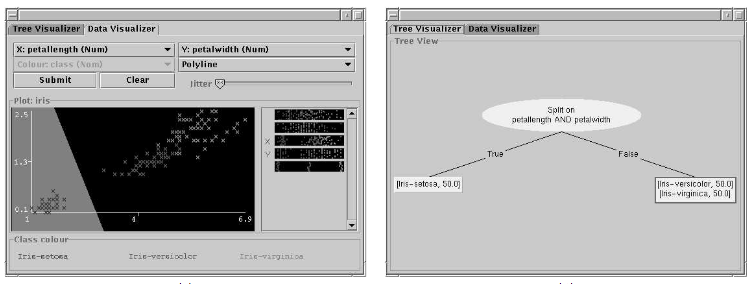
\includegraphics[width=1\textwidth]{dtreeconstructor}
\caption{\textbf{Decision Tree Constructor} The user chooses the attributes to display on the axes and draws a polyline to enclose an area. In the tree visualizer, the examples in the enclosed are in the left node and the rest of the examples are in the right node. }\label{fig:dtreeconstructor}
\end{figure}

Ware et al. \cite{InteractiveML} created a system for interactive decision tree construction as shown in figure \ref{fig:dtreeconstructor}. The system captures the interaction between pairs of attributes in two-dimensional visualizations. The user chooses attributes to display on the axes of the scatter plot and draws a polygon to enclose an area that will define the split. When the user submits the visual, and the tree inserts two new nodes, one containing the examples in the split and the other receives the rest of the examples. The tree is also visualized by the system. The system was evaluated by having five novice users construct decision trees for five standard datasets from UCI and comparing the accuracy of the human-system generated decision trees to those generated by C4.5, a standard decision tree algorithm. Their results show that the users' trees are smaller and performed better than those constructed by C4.5 for three of the five datasets. 

\begin{figure}[h]
\centering
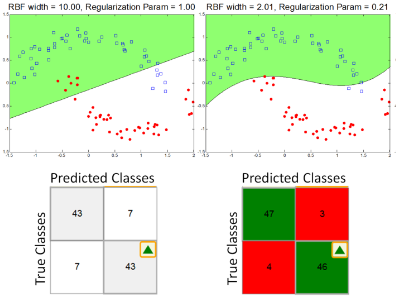
\includegraphics[width=1\textwidth]{manimatrix}
\caption{ \textbf{ManiMatrix.} ManiMatrix can be used to learn kernel parameters that would result in a model that will have the performance desired by the user. In this example, the RBF kernel width and regularization parameter update to correspond to the interactive confusion matrix. The top decision boundary corresponds to the bottom state of the confusion matrix. }\label{fig:manimatrix}
\end{figure}

ManiMatrix is an interactive system that enables users to align the classifier's behavior with their desired performance. \cite{ManiMatrix}. For example, the user may prefer a classifier with a low false positive rate than other models with similar performance. ManiMatrix uses humans to guide the exploration and learning of a kernel and its hyperparameters for multiclass classification. The user expresses their preference by incrementing or decrementing the cells of an interactive confusion matrix. The interactions determine how the algorithm explores the solution space. Updates to the kernel parameters and decision boundary updates correspond to the confusion matrix as shown in figure \ref{fig:manimatrix}. Their system enables people to guide the exploration of possible models in accordance with their preferences. 

\begin{figure}[h]
\centering
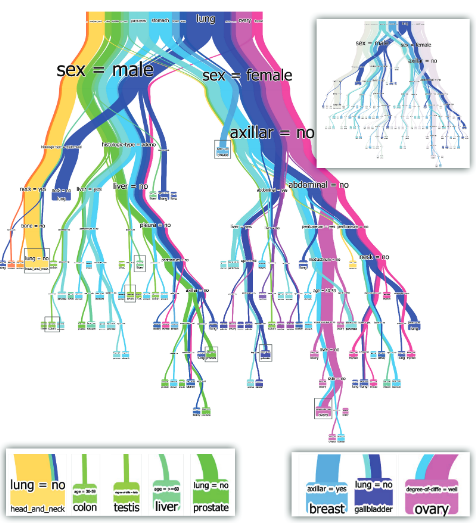
\includegraphics[width=1\textwidth]{baoview}
\caption{\textbf{BaobabView.} This example is used to describe how BaobabView can be used to explore and analyze datasets. The dataset used is a medical dataset to determine the location of primary tumors. The tree first splits on sex. Typical diagnoses for males show on the lower left and females on the lower right. The upper right shows diagnoses common to both.}\label{fig:baoview}
\end{figure}

Interactive visual systems have also been created for specific machine learning models or structures such as decision trees and neural networks. For example, BaobabView \cite{BaobabView} visualizes the construction and analysis of decision trees. The decision tree is represented as a node-link diagram where nodes represent features and the width of links are proportional to the number of items going from their parent to their child node. The system designed interactions to allow the user to bring in prior knowledge. The user can choose the most significant feature as the first feature to split the dataset and also which leaf nodes in the resulting tree to split further. The authors demonstrate the effectiveness of the system by presenting two use cases. The first shows the interactive decision tree construction process including growing and pruning the tree using an outdoor image segmentation dataset. The second use case demonstrates the effectiveness and scalability of the system's design for analyzing datasets as shown in figure \ref{fig:baoview}. The authors did not present an evaluation study; the system's interface has many components and possible user study participants may need more time to be familiarized with the system. In contrast, our goal is to create intuitive interactions and visuals that are easy to analyze, such that users with basic knowledge of machine learning would quickly be onboard.

Visual analytic tools where users can interactive construct or develop machine learners have also been developed for classification of text documents \cite{ClassifyText}, logistic regression models \cite{LogReg}, topic modeling \cite{TopicModeling}.

\subsection{ Model Analysis }
Visual analytic techniques have been employed to understand model behavior and interpret predictions. In order to fully leverage the power of deep learning and employ them in real life situations, domain experts need to first understand and explain the model's predictions. Visual analytics approaches have been implemented for various types of deep learning models - for example, recurrent neural networks \cite{RetainVis}, deep Q-Networks \cite{DQNViz}, deep neural networks \cite{UnderstandingNN}, and convolutional networks \cite{CNN}. 

Krause et al. implemented Rivelo \cite{Tamagnini}, an interactive explanation interface for exploring instance level explanation, which the authors defined as the set of features that explain the prediction of an example. The interface is comprised of a list of feature ranked according to how frequent the feature appeared in instance explanations and also of visual representations of the feature vectors that explain the examples. The authors conducted a case study involving medical experts to showcase how the system supports diagnostic analysis of complex machine learning models. Other visual analytics tools developed for interpreting machine learning include Prospector \cite{Prospector} for making sense of predictive models 

\subsection{Model Diagnosis}
Another major goal of integrating visual analytic techniques and learning models is to diagnose models. Commonly used simple summary statistics for analyzing performance do not help users identify outliers, diagnose problems in the data set, or provide insights on how to improve the current model in the next iteration. Various diagnostic systems have been proposed and implemented.

\begin{figure}[h]
\centering
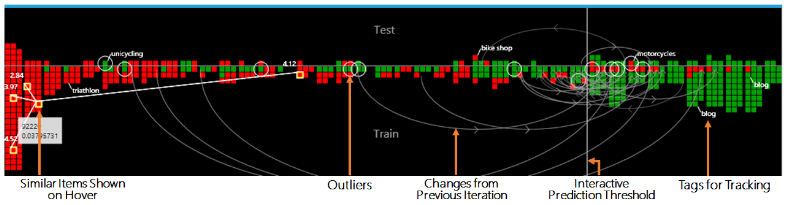
\includegraphics[width=1\textwidth]{ModelTracker}
\caption{\textbf{ModelTracker.} ModelTracker visually conveys model performance and also enables the user to inspect the data. Green boxes are correctly predicted examples, while red boxes are falsely predicted examples. Since low scoring examples are to the left and high scoring examples are to the right, a high performing model will have most green boxes to the right and most red boxes to the left. Users can click on boxes to directly interact with individual data points and flag examples that may be outliers or falsely mislabeled.  }\label{fig:ModelTracker}
\end{figure}

ModelTracker \cite{ModelTracker} (figure \ref{fig:ModelTracker}) is another example of a visual system for performance or diagnostic analysis of binary classification. Each example is represented by a square box where the color green codes for accurate predictions and red codes for false prediction. The boxes are laid horizontally from low to high prediction scores for the true class, so a high performing model will have mostly green squares on the right end and red squares on the left end. The visual communicates prediction scores, the overall performance of the model and outliers in the data set and enables users to debug model predictions. The author evaluated their system by observing seven machine learning practitioners interacting with the system as they built their binary classification model and identifying a common usage strategy and common user interactions. 

\begin{figure}[h]
\centering
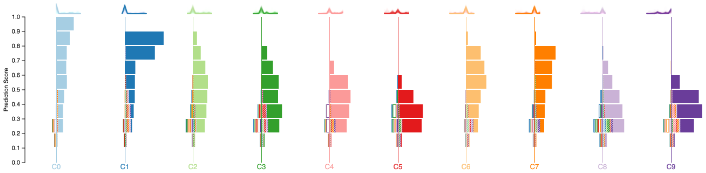
\includegraphics[width=1\textwidth]{Squares}
\caption{\textbf{Squares.} Squares is a performance analysis tool that displays histograms of prediction scores for each target label. The histograms show the distribution of prediction scores, and help users identify severe errors such as false positives with a high prediction score. }\label{fig:Squares}
\end{figure}

A different design for visualizing performance analysis of multiclass classification is Squares \cite{Squares} (figure \ref{fig:Squares}). For each class, a histogram displays the distribution of prediction scores which cannot be communicated in common statistical measures. The color of the bar represents the true target label. True positives are distinguished from false positives and false negatives by the pattern of the histogram bar. Squares is agnostic to common performance metrics and helps connect model performance to the data. The authors verified their design through a user study where participants completed tasks that require them to interact and interpret the visuals. The evaluation showed that participants are able to visually assess the performance of the classifier and identify more severe errors such as false positives with high scores and examples of a class that are consistently confused by the classifier for being of another class.

Other related works in visualizing results of machine learning include iVisClassifier \cite{iVisClassifier} for classification models and iPCA \cite{iPCA} for dimensionality reduction of datasets.

\subsection{Visualizing for Feature Selection}
\begin{figure}[h]
\centering
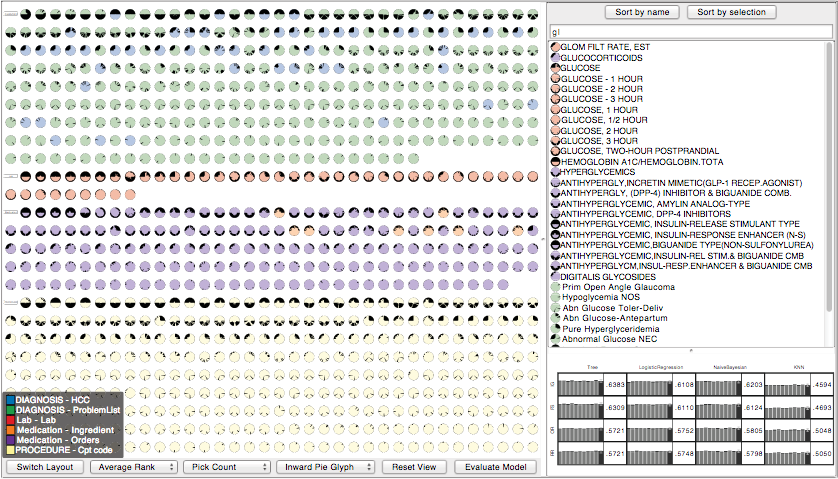
\includegraphics[width=1\textwidth]{INFUSE}
\caption{ \textbf{INFUSE.} A feature selection visualization. Each circle represents a feature. The features are ranked according to its predictive power determined across various feature selection algorithms. }\label{fig:INFUSE}
\end{figure}

\indent A common strategy for visualizing high dimensional data is to reduce dimensions so the data can be visualized in one, two, or three-dimensional space. Non-traditional methods of applying dimensional reduction have been implemented and utilize visualization. Guo \cite{Guo} implemented an interactive feature selection approach that uses visuals to identify patterns in feature subspaces. Every pair of features is represented in a colored matrix where the color codes for pair-wise similarity. The matrix is sorted to highlight interesting clusters in feature subsets, and users can reduce the set of features to display. The authors demonstrated the properties of their system by describing a use case featuring a dataset for predicting breast cancer rate in a county based on attributes of the county. No further evaluation study using participants is described.  

Fernstad and Johansson also implemented an interactive dimensionality reduction strategy that utilizes visualization \cite{InteractiveDR}. The user chooses metric the system uses to rank the features and the number of ranked features to display in a parallel coordinate visual or scatterplot matrix. The user can also rank pairs of features and inspect a matrix of feature pairs to identify interesting relationships.

INFUSE \cite{INFUSE} (figure \ref{fig:INFUSE}) is an interactive feature selection system that can be used to rank feature and compare prediction models resulting from different feature selection algorithms. INFUSE uses the outputs of multiple feature selection algorithms to display the ranking of features according to their estimate predictive power. In our approach, we do not explicitly tell the user which features are predictive, instead, we use visuals of prior knowledge to guide users towards a predictive feature set. Similar to our design features are the primary data items of INFUSE. 

Both INFUSE and our approach interactive allows the user to explore the feature space and select features. However, INFUSE is based on using information about features obtained from common feature selection methods while our approach is based on helping the user utilize their prior knowledge and using causality to determine predictive feature sets. INFUSE represents a feature as a glyph which is divided into quadrants visualizing the predictive power of the feature using each of the four feature selection algorithms. The purpose of the glyph is to visualize the predictive power of a feature according to four different algorithms. In contrast, we represent a feature as an axis and include data about feature values in order to visualize the correlation between feature values. INFUSE provides prediction models that result from well-known feature selection algorithms and allows the user to create their own models and compare their custom model to the system created models. Our system also allows the user to compare the model created using one feature set against other models created using different feature sets; our system provides one default model created using prior knowledge the user provides.

The authors evaluated their system through a case study. Clinical researchers learn about the capabilities of the system and used INFUSE to explore features for creating a model to predict patients at high risk of developing diabetes. The researchers provided feedback on the system, and many mentioned that INFUSE gave them the opportunity to examine multiple algorithms at the feature-level. Each feature selection algorithm captures different types of information, and INFUSE enables the experts to see the outcome of that information being captured. INFUSE gives the user the power to merge features from different algorithms and shows promise of improving the predictive models of experts.
